% Drawing 43/03-1 -- folder 43, batch 03, archive page 54 (PDF page 55).
% Transcription: à gauche, des croquis de segments subdivisés, avec les légendes :
% Kind: two subdivided segments. Method 2 (schematic redraw from the facsimile). Status: ok.
% Notes: Two horizontal segments: the first with heavy end ticks, a small tick and a crossed point marked with a small v above; the second with heavy ticks near both ends and a small tick beyond. The legends are text after the mark.
% Coordinates: 1 unit = 1 mm = 1/100 of the crop width (bbox in page fractions: [0.05, 0.47, 0.4, 0.6]).
% Redrawn by Claude (claude-opus-5-5), issue #73, 2026-11-07; not checked by a human; not compiled (no TeX in the session).
% Rights: reproduces part of the work -- behind RENDER_TRANSCRIPTS, never published by itself.
\documentclass[tikz,border=3pt]{standalone}
\usepackage{amsmath,amssymb}
\usetikzlibrary{patterns,arrows.meta}
\tikzset{pencil/.style={black!45}, struck/.style={black!35}, mark/.style={circle,draw,inner sep=1.3pt}, pt/.style={circle,fill,inner sep=0.9pt}, opt/.style={circle,draw,fill=white,inner sep=1.1pt}}
\begin{document}
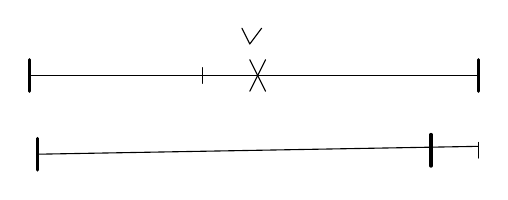
\begin{tikzpicture}[x=1mm,y=1mm,line cap=round,line join=round,font=\scriptsize]
\draw (33,-30) -- (90,-30);
\draw[very thick] (33,-28) -- (33,-32);
\draw[very thick] (90,-28) -- (90,-32);
\draw (55,-29) -- (55,-31);
\draw (61,-28) -- (63,-32);
\draw (63,-28) -- (61,-32);
\draw (60,-24) -- (61,-26) -- (62.5,-24);
\draw (34,-40) -- (90,-39);
\draw[very thick] (34,-38) -- (34,-42);
\draw[very thick] (84,-37.5) -- (84,-41.5);
\draw (90,-38.5) -- (90,-40.5);
\end{tikzpicture}
\end{document}
